\usepackage{fullpage}

\section{Discovering Communities in MetaFilter}

Asim Ihsan
\emph{\textless{}\href{mailto:asim.ihsan@gmail.com}{\texttt{asim.ihsan@gmail.com}}\textgreater{}}\\7th
November 2012

\subsection{1. Abstract}

MetaFilter is an active and exciting online forum that discusses topics
from politics to poetry, culture to computing. Running since 1994, it
allows members to post topics onto a front page, comment on the topics,
and mark both posts and comments as ``favorites''. In this paper I
discuss several hypotheses surrounding these participation mechanisms,
how I collected data to investigate these hypotheses, and what methods I
used to test my hypotheses. My conclusion is that there is clear
evidence that several small-world communities are present on MetaFilter.

Section 2 clarifies what parts of MetaFilter I am seeking to analyse,
what hypotheses I wish to test, and why I think these hypotheses are
interesting. Section 3 explores the gathered data with several metrics,
compares them to Erdős--Rényi graphs of the same size, and draws
conclusions. Section 4 addresses limitations of my approach and
suggested areas for future work.

\subsection{2. MetaFilter, hypotheses, and data collection}

\subsubsection{MetaFilter}

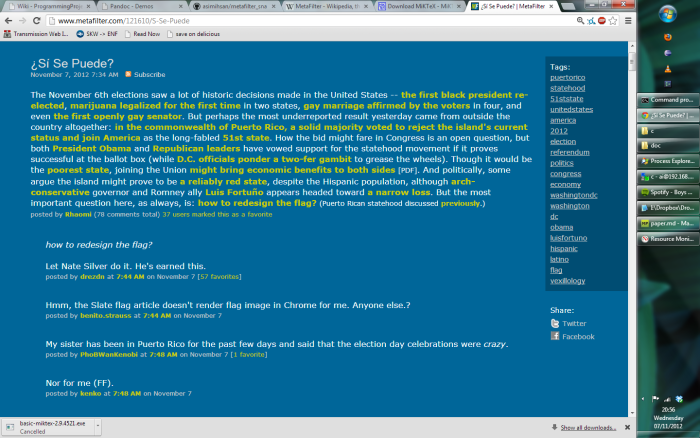
\includegraphics{01_metafilter_screenshot.png}~

MetaFilter is an online forum where members are free to post on whatever
they want. You'll notice in the screenshot above two important points:

\begin{itemize}
\item
  Users can \textbf{mark a post as a favorite}. Using this mechanism
  means that the post is explicitly marked as a user's favorite in their
  profile page.
\item
  Users can \textbf{post comments} and have those comments themselves
  marked as favourites.
\end{itemize}

\subsubsection{Hypotheses}

Although users have their own particular motivations for participating
in online forums I believe that they do so in a context that largely
reinforces their own beliefs, values, and finite interests. MetaFilter
regularly hosts an astonishingly wide variety of topics, however I want
to test to what extent people segregate their time and attention to
particular subtopics, if at all.

Hence, the hypotheses I wish to test are:

\begin{itemize}
\item
  \textbf{H1}: Users will tend to both favorites posts and comment on
  posts with particular subsets of the total set of users.
\item
  \textbf{H2}: Users are less likely to focus their favorites as they
  are their comments.
\end{itemize}

Intuitively, H1 is likely to be true because users each have their own
interests and these are likely to intersect with strict subsets of other
users. Attention and time are so finite that we're likely to behave like
this. Given how broad the topic variation is on MetaFilter it'd be
interesting to see what these topic clusters are.

H2 is a bit more obscure but perhaps more interesting. I believe there
is a significantly lower threshold to ticking a single link marking a
post as a favorite, perhaps marking it for later reading or reference,
than there is to actively commenting on a post. The latter is so much
more involved and time consuming that users, perhaps, will restrict such
an action to those topics which they are particularly interested in.

\subsubsection{Data collection}

In short the code I've written uses Python to launch a small number of
workers to scrape posts off of MetaFilter. They output an SQLite
database with a single table, ``posts'', with the raw HTML required for
subsequent analysis.

You may find the code that I've used to collect and parse the data in
the following GitHub repository:

\url{https://github.com/asimihsan/metafilter_sna}

Here are some basic instructions on setting up your computer to execute
this code. These instructions have only been testing on Mac OS X but the
equivalent Linux instructions (i.e.~using \texttt{yum} or \texttt{apt})
should work.

Please note that these instructions are very rough and are untested. If
you encounter any difficulties please feel free to contact me via GitHub
for help, I'm happy to assist.

\begin{itemize}
\item
  Mac OS X

  \begin{itemize}
  \item
    Install Homebrew (\url{http://mxcl.github.com/homebrew/})
  \item
    Install RabbitMQ using Homebrew
    (\url{http://www.rabbitmq.com/install-homebrew.html})
  \item
    Install Python 2.7 and virtualenv using Homebrew
    (\url{https://gist.github.com/1208841})
  \item
    Checkout the code from the git repository above.
  \item
    Create a new virtulenv for this code:

\begin{verbatim}
mkvirtualenv metafilter_sna
\end{verbatim}
  \item
    Install the dependencies for the repository:

\begin{verbatim}
pip install -r requirements.txt
\end{verbatim}
  \item
    In one terminal window execute the celery workers:

\begin{verbatim}
cd metafilter_sna/src/01_scrape/
./launch_celeryd.sh
\end{verbatim}
  \item
    In a second terminal window execute the following to monitor the
    celery workers to confirm that they are working:

\begin{verbatim}
cd metafilter_sna/src/01_scrape/
celeryev -A tasks
\end{verbatim}
  \item
    In a third terminal window execute the trigger script that starts
    the scraping:

\begin{verbatim}
cd metafilter_sna/src/01_scrape/
./main.py
\end{verbatim}
  \item
    On executing \texttt{main.py} you should notice both the first two
    terminal windows outputting a lot of logs. If not something is
    wrong!
  \item
    After gathering a sufficient amount of data you can execute the
    following in order to convert the SQLite database into the pair of
    GML graph files:

\begin{verbatim}
cd metafilter_sna/src/02_parse
./database_to_gml.py
\end{verbatim}
  \item
    The above script will output GML files into the ``data''
    subdirectory.
  \end{itemize}
\end{itemize}

\subsubsection{Nodes, edges, weights}

In this paper we will create \textbf{weighted, undirected} graphs where
nodes are \textbf{users}. We will use the data collected above to create
two graphs:

\begin{itemize}
\item
  \textbf{Favorites}: a graph where an edge exists between two users if
  they have favorited the same post. The weight of the edge is
  $ln(x+1)$, where $x$ is the number of posts co-favorited.
\item
  \textbf{Comments}: a graph where an edge exists between two users if
  they have commented on the same post. The weight of the edge is
  $ln(x+1)$, where $x$ is the number of posts co-commented.
\end{itemize}

\subsection{3. Data analysis and conclusions}

For this paper I will consider the last 1,386 posts on MetaFilter,
covering a time period of approximately one and a half months. Both the
SQLite database of raw HTML, discussed in section 2, and the Graph
Markup Language (GML) files of the corresponding weighted undirected
graphs are available in the following compressed 7-Zip file here:

\url{http://aifiles.s3.amazonaws.com/metafilter_sna_data.7z}

Table 1 summarises metrics for the favorites graph, described in section
2, in comparison to an Erdős--Rényi graph with he same number of nodes
and edges:

\begin{tabular}{|l|l|l|}\hline
Metric & Favorites graph & Erdős–Rényi graph \\ \hline
Nodes  & 3,693 & 3,963 \\
Edges  & 329,288 & 329,576 \\
Average clustering coefficient & 0.315 & 0.0482 \\
Diameter & 4 & 3 \\
Average shortest path length & 2.00 & 1.95 \\
Number of communities via greedy optimization of modularity & 13 & 5 \\
Largest community via greedy optimization of modularity & 1831 & 1429 \\
Number of communities via walktrap & 43 & 9 \\
Largest community via walktrap & 2304 & 723 \\
\end{tabular}

The following is interesting about the above:

\begin{itemize}
\item
  Compared to a similar ER graph, i.e.~a graph with a similar number of
  edges and nodes where edges connect at random, the favorites graph has
  a higher average clustering coefficient. This means that, on average,
  each node in the favorites graph is closer to becoming a
  \emph{clique}, i.e.~a complete subgraph, than a random graph. This
  suggests that clustering is more common than random in the favorites
  graph.
\item
  Compared to a similar ER graph the favorites graph has a similar
  average shortest path length. The combination of a relatively high
  average clustering coefficient and similar average shortest path
  length suggests the favorites graph is exhibiting \emph{small-world}
  behavior, i.e.~that there are tightly-bound and very connected
  subgraphs, and the subgraphs are sparsely connected to other
  subgraphs.
\item
  Using two methods for approximating the number of communities in the
  graph, either by maximizing modularity or using random walks
  (i.e.~walktrap), we see that there are more communities present than
  random and that the largest community is larger than random.
\end{itemize}

Table 2 summarises metrics for the comments graph, described in section
2, in comparison to an Erdős--Rényi graph with he same number of nodes
and edges:

\begin{tabular}{|l|l|l|}\hline
Metric & Comments graph & Erdős–Rényi graph \\ \hline
Nodes  & 4,348 & 4,348 \\
Edges  & 749,313 & 748,481 \\
Average clustering coefficient & 0.468 & 0.0792 \\
Diameter & 4 & 2 \\
Average shortest path length & 1.97 & 1.92 \\
Number of communities via greedy optimization of modularity & 11 & 3 \\
Largest community via greedy optimization of modularity & 3460 & 1926 \\
Number of communities via walktrap & 16 & 10 \\
Largest community via walktrap & 3405 & 758 \\
\end{tabular}

As the metrics for the comments graph relative to an equivalent random
graph are remarkably similar I will not regurgitate the same conclusions
that have already been discussed.

Table 3 compares metrics between the comments and favorites graphs:

\begin{tabular}{|l|l|l|}\hline
Metric & Comments graph & Favorites graph \\ \hline
Nodes  & 4,348 & 3,693 \\
Edges  & 749,313 & 329,288 \\
Average clustering coefficient & 0.468 & 0.315 \\
Diameter & 4 & 4 \\
Average shortest path length & 1.97 & 2.00 \\
Number of communities via greedy optimization of modularity & 11 & 13 \\
Largest community via greedy optimization of modularity & 3460 & 1831 \\
Number of communities via walktrap & 16 & 43 \\
Largest community via walktrap & 3405 & 2304 \\
\end{tabular}

In comparing the comments and favorites graphs note that the comments
graph is not only more clustered but also has less communities, with the
largest community is greater than that of the favorites graph.

\subsubsection{Calculation}

Before stepping into the interpretation and conclusions I'd like to go
over how the above metrics were calculated.

I used R and the igraph package to calculate all of the above metrics.
Here is a script that calculates all of the above:

\begin{verbatim}
library(igraph)
library(ggplot2)

g = read.graph("I:\\Programming\\metafilter_sna\\data\\comments.gml", format="gml")

# Number of nodes and edges.
summary(g)

# Average clustering coefficient.
transitivity(as.undirected(g))

# Diameter.
diameter(g)

# Average shortest path.
average.path.length(as.undirected(g))

# Community finding using greedy optimization of modularity.
fc = fastgreedy.community(as.undirected(g))    
fc_sizes = sizes(fc)
max(fc_sizes)

# Community finding using greedy optimization of modularity.
wt = walktrap.community(as.undirected(g))
wt_sizes = sizes(wt)
max(wt_sizes)
\end{verbatim}

In order to derive the equivalent random graph metrics you can generate
an Erdős--Rényi graph with the same number of nodes and then calculate
an appropriate edge probability $p$ such that:

$\frac{N(N-1)}{2} \times p = E$

Where N is the number of nodes, E is the number of edges. Generating the
graph is as simple as substituting the \texttt{g} line above with:

\begin{verbatim}
g <- erdos.renyi.game(N, p)
\end{verbatim}

\subsubsection{Interpretation and conclusions}

(Please note that I have not provided a visualization of my data because
I was unable to find a suitable layout algorithm that displayed anything
useful!)

I believe that the above results confirm hypothesis H1, i.e.~that users
tend to both favorite posts and comment on posts wuth particular subsets
of other users, i.e.~in clusters. Both the average clustering
coefficients and the community finding algorithms confirm this.
Moreover, and even more interesting, with the average shortest paths the
same between both the favorites and comments graphs and their equivalent
ER graphs, it's clear that there is small-world structure in effect.

I also belive that the results confirm hypothesis H2, i.e.~that users
are more discriminative and clustered on high-effort participation
methods. However, to what degree is difficult to say. Is an average
clustering coefficient $0.468 > 0.315$ sufficient to say that comments
graphs are ``more clustered'' than favorites graphs? If so then to what
extent? This is very difficult to say. However I think that, in
combination with the larger community sizes, the comments graph seems to
be ``more community like'' than the favorites graph.

\subsection{4. Limitations and suggestions for future work}

There are a wide variety of limitations to the above that should be
mentioned:

\begin{itemize}
\item
  The weighting of the edges is rather arbitrary. Why $ln(x+1)$? Simply
  because I did not want users who have co-favorited 2 posts to be twice
  as important as those who have co-favorited 1. I think a logarithmic
  weighting is appropriate and that the constant factor is negligible,
  but this is an assumption.
\item
  I did not collect that much data. \textasciitilde{}1,300 posts is not
  enough. However, I've set up my scraping scripts to be very slow in
  order to be polite to the MetaFilter system administrators; more data
  could yield a more clear confirmation of e.g.~hypothesis H2.
\item
  An overlapping community detection algorithm seems quite ideal here,
  and should be applied in future studies.
\end{itemize}
